\documentclass{slides}
\usepackage{geometry,color}
\usepackage{graphicx} % Required for inserting images
\usepackage[font=small,labelfont=bf]{caption} % Required for specifying captions to tables and figures
\usepackage{amsmath}
\usepackage{amssymb}
\usepackage{cite}
\usepackage{algorithm}
\usepackage{algpseudocode}
\usepackage{biblatex}
\usepackage{float}
\usepackage{hyperref}

\geometry{screen}
\paperwidth 11.0truein
\paperheight 8.5truein
\oddsidemargin -0.25truein
\evensidemargin -0.25truein
\textheight 7in
\textwidth 9.5in
\topmargin -.8in


\newcommand{\R}{\mathcal{R}}
\newcommand{\U}{\mathcal{U}}
\newcommand{\PA}{\mathcal{P}}
%\usepackage{makeidx,multicol,cite,verbatim}
%\usepackage{amsmath,amssymb,amscd,fixmath,upgreek,amsthm,textcomp}
%\usepackage[mathscr]{eucal}% \makeindex
%\usepackage{Mngr-sli}
%\usepackage{Mngr-macros-sli}
%\raggedbottom
%%%%%%%%%%%%%%%%%%%%%%%%%%%%%%%%%%%%%%%%%%
\definecolor{dmagenta}{rgb}{.4,.1,.5}
\definecolor{007}{rgb}{.0,.0,.7}
\definecolor{dred}{rgb}{.5,.0,.0}
\definecolor{dgreen}{rgb}{.0,.5,.0}
\definecolor{dblue}{rgb}{.0,.0,.5}

\definecolor{550}{rgb}{.5,.5,.0}
\definecolor{505}{rgb}{.5,.0,.5}
\definecolor{055}{rgb}{.0,.5,.5}
\definecolor{551}{rgb}{.5,.5,.1}
\definecolor{515}{rgb}{.5,.1,.5}
\definecolor{155}{rgb}{.1,.5,.5}

\definecolor{400}{rgb}{.4,.0,.0}
\definecolor{040}{rgb}{.0,.4,.0}
\definecolor{004}{rgb}{.0,.0,.4}
\definecolor{440}{rgb}{.4,.4,.0}
\definecolor{404}{rgb}{.4,.0,.4}
\definecolor{044}{rgb}{.0,.4,.4}
\definecolor{441}{rgb}{.4,.4,.1}
\definecolor{414}{rgb}{.4,.1,.4}
\definecolor{144}{rgb}{.1,.4,.4}

\definecolor{300}{rgb}{.3,.0,.0}
\definecolor{030}{rgb}{.0,.3,.0}
\definecolor{003}{rgb}{.0,.0,.3}
\definecolor{330}{rgb}{.3,.3,.0} %
\definecolor{303}{rgb}{.3,.0,.3}
\definecolor{033}{rgb}{.0,.3,.3}
\definecolor{331}{rgb}{.3,.3,.1}
\definecolor{313}{rgb}{.3,.1,.3}
\definecolor{133}{rgb}{.1,.3,.3}

\definecolor{200}{rgb}{.2,.0,.0}
\definecolor{020}{rgb}{.0,.2,.0}
\definecolor{002}{rgb}{.0,.0,.2}
\definecolor{220}{rgb}{.2,.2,.0} %
\definecolor{202}{rgb}{.2,.0,.2}
\definecolor{022}{rgb}{.0,.2,.2}
\definecolor{221}{rgb}{.2,.2,.1}
\definecolor{212}{rgb}{.2,.1,.2}
\definecolor{122}{rgb}{.1,.2,.2}

\definecolor{violet}{rgb}{.3,.0,.9}
\definecolor{orange}{cmyk}{0,.5,.1,.0}
\definecolor{dcyan}{cmyk}{.5,.0,.0,.0}
\definecolor{dyellow}{cmyk}{.0,.0,.5,.0}
\definecolor{cm}{cmyk}{1,.0,.0,.0}
\usepackage{graphicx}

% red,blue,yellow,magenta,cyan,green,black



%%%%%%%%%%%%%%%%%%%%%%%%%%%%%%%%%%%%%%%%%%
\title{\color{007}\Large Lagrangian index for restless bandits}\author{\large Vivek S.\ Borkar\\
IIT Bombay}\date{\large Google Research, Bengaluru\\ 18th March, 2024}
%%%%%%%%%%%%%%%%%%%%%%%%%%%%%%%%%%%%%%%%%%
\begin{document}
\maketitle
%%%%%%%%%%%%%%%%%%%%%%%%%%%%%%%%%%%%%%%%%%
%%%%%%%%%%%%%%%%%%%%%%%%%%%%%%%%%%%%%%%%%%
\newpage

{\large \color{dblue}

\textbf{Restless bandits:}

$N$ controlled Markov chains $X^i_n, n \geq 0,$  on a finite state space $S$ for $1\leq i \leq N$, with two possible modes: {\color{red} active} and {\color{red} passive}, corresponding to control choices $1$ and $0$ resp.

Let $U^i_n \in \{0,1\}$ denote the control choice for arm $i$ at time $n$.

Transition probabilities $p_u^i(k|j)$, rewards $r^i_u(j)$ for $j,k \in S$ and control $u^i\in\{0,1\}$ with $u^i = 1 \Leftrightarrow$ active mode.

\newpage

The problem then is to choose the controls $U^i_n \in \{0,1\}$ for arm $i$, $1\leq i \leq N$ so as to maximize
$$\lim_{n\to\infty}\frac{1}{n}E\left[\sum_{m=0}^{n-1}\sum_{i=1}^Nr^i_{U_n}(X^i_n)\right]$$
subject to the constraint $\sum_{i=1}^NI\{U^i_n=1\} = M$
for a\\ prescribed $M < N$.

Here $I\{\cdots\} = 1$ if `$\cdots$' is true, $0$ otherwise, is the indicator function,

$p_0(j|i) = \delta_i(j)$ corresponds to the classical multi-armed (rested) bandit, optimal index policy known\\ (Gittins index).

\newpage

Restless bandit problem is provably hard, only a heuristic index policy due to Whittle is known. This is motivated by the Lagrangian formulation after relaxing the per time constraint
$$\sum_{i=1}^NI\{U^i_n=1\} = M$$
to the average constraint
$$\lim_{n\to\infty}\frac{1}{n}E\left[\sum_{m=0}^{n-1}\sum_{i=1}^NI\{U^i_m=1\}\right] = M.$$
Then this is the classical {\color{red} `constrained Markov decision process'} which admits the Lagrangian formulation of maximizing the unconstrained reward
$$\lim_{n\to\infty}\frac{1}{n}E\left[\sum_{m=0}^{n-1}\sum_{i=1}^N\left(r_{U_m}(X^i_m) + \lambda^*\left(I\{U^i_m=1\} - \frac{M}{N}\right)\right)\right].$$

\newpage

Given $\lambda^*$, this is a separable problem that seeks to\\ maximize for the $i$th arm
$$\lim_{n\to\infty}\frac{1}{n}E\left[\sum_{m=0}^{n-1}\left(r^i_{U_m}(X^i_m) + \lambda^*\left(I\{U^i_m=1\} - \frac{M}{N}\right)\right)\right].$$
 
The Whittle heuristic, motivated by the above, is as follows. Consider a single arm, say the $i$th. Add a `subsidy' $\lambda \in \R$ to $r_0(\cdot)$ to encourage passivity. 

The problem is said to be {\color{red} (Whittle) indexable} if under the optimal policy, the set of passive arms increases from the empty set to $S$ as $\lambda$ increases from $-\infty$ to $+\infty$ \\\textbf{monotonically}. 

\newpage

If so, define the {\color{red} Whittle index} $\lambda^i(j)$ for arm $i$ for state $j\in S$ to be the value of $\lambda$ for which active or passive mode is equally preferable over  for state $j$ and arm $i$. \\
Recall the dynamic programming equation for the value function $V^i: S \mapsto \R$ and the optimal cost $\beta^i$:
\begin{eqnarray*}
V(j) &=& \max_u\Big[u(r_1^i(j) + \sum_kp_1^i(k|j)V(k)) + \\
&&(1-u)(r_0^i(j) + \lambda + \sum_kp_0^i(k|j)V^i(k)\Big] - \beta^i.
\end{eqnarray*}
Then $\lambda^i(j) := Q^i(j,1) - Q^i(j,0)$ where,
$$Q^i(j,u) := r^i_u(j) + \sum_kp^i_u(k|j)V^i(k), \ u\in\{0,1\}.$$

\newpage

The Whittle heuristic then is to sort arms at time $n$ according to the decreasing order of $\lambda(X^i_n)$ and set the first $M$ active, resolving any ties probabilistically.

This reduces to Gittins index for rested bandits (Whittle). It is optimal in an asymptotic sense for identical arms (Weiss and Weber). 

It has been found useful in many scheduling applications, such as web crawling, congestion control, machine maintenance, cloud computing. AoI aware scheduling, etc.

\newpage

One common strategy for proving Whittle indexability is to view the value function as a function of state $x$ and subsidy $\lambda$.\\
First, prove monotonicity, convexity etc., which leads to the existence of an optimal threshold policy wherein the threshold depends on the parameter $\lambda$.\\
Then prove  the `increasing differences' property:\\ for $y>x, \lambda'>\lambda$,
$$V(y,\lambda') - V(x,\lambda') \geq V(y,\lambda) - V(x-\lambda).$$
This leads to monotne dependence of the threshold on $\lambda$. This leads in turn to Whittle indexability.


\newpage

\textbf{Q-learning for Whittle index (Avrachenkov, Borkar (Automatica 2022))}

For each $i\in S$, run a Q-learning algorithm for average cost with subsidy $\lambda$, based on relative value iteration (Abounadi, Bertsekas, Borkar 2001) to obtain $Q_n^i(j,u) \to \bar{Q}^i_\lambda(j,u)$.

Compute the Whittle index by solving for $\lambda = \bar{Q}^i_\lambda(i,1) - \bar{Q}_\lambda^i(i,0)$, by iterating
$$\lambda_{n+1} = \lambda_n + b(n)(Q^i_n(i,) - Q^i_n(i,0)).$$

\newpage

To reduce computation, it suffices to compute the index for a sufficiently representative subset of $S$ and interpolate (easy for ordered state spaces).

Index policies use {\color{red} ordinal comparisons}, hence are robust. So good approximations suffice.

Nevertheless, for large problems, function approximations are needed. These  interpolate between states automatically.

Several works take this approach:

\newpage

Fu, Nazarathy, Moka (Australian and New Zealand Control Conf., 2019)\\
Nakhleh, Ganji, Hsieh, Hou, Shakkottai (Neurips 2021)\\
Gibson et al (EAI Performance Eval.\ Methodologies and Tools  2021)\\
Robledo, Borkar, Ayesta, Avrachenkov (Euro.\ Workshop on RL, 2022)\\
Xu, Taneja, Tambe (preprint 2022)\\
Akbarzadeh, Mahajan (IEEE TCNS 2023)

Nevertheless, the problem remains computation-heavy.
}

\newpage

{\large \color{dred}

\textbf{Alternative approach: Lagrange index}

Go to the classical Lagrangian formulation: since the primary and secondary rewards are separable, the problem decouples into $N$ individual problems of maximizing
$$\lim_{n\to\infty}\frac{1}{n}E\left[\sum_{m=0}^{n-1}\left(r_{U^i_m}(X^i_m) + \lambda^*\left(I\{U^i_m = 1\} - \frac{M}{N}\right)\right)\right].$$
for $1\leq i \leq N$. Let $Q^i(j,u), j \in S, u \in \{0,1\}$, denote the corresponding Q-values, computable by the Q-learning algorithm based on relative value iteration.

The {\color{red} Lagrange index} for state $i \in S$ then is 
$$\lambda(i) := Q^i(i,1) - Q^i(i,0).$$

\newpage

The {\color{red} Lagrange index policy} is to sort the Lagrange indices $\{\lambda(X^i_n\}$ at time $n$ in decreasing order and pick he top $M$, resolving any tie by randomization.

\textbf{Advantages:}

1.\ No separate iteration is required for index calculation.

2.\ As for Whittle indices, it involves ordinal comparison, hence robust.

\newpage

Brown, Smith (Management Science 2020)\\
Zhang and Frazier (preprint 2022)\\
Killian, Biswas, Shah and Tambe (27th ACN SIGKDD 2021)\\

\newpage

We next prove the asymptotic optimality of the Lagrange index policy. We begin with some simple lemmas.

Let $P, P_0$ be irreducible stochastic matrices on a finite state space $S, |S| = s$, with invariant distributions $\pi,\pi_0$ resp., both viewed as row vectors.
Let $\epsilon, \epsilon' > 0$.

\textbf{Lemma 1} If $\|P-P_0\|_\infty \leq \epsilon$, then:

1.\  $\|\pi-\pi_0\|_\infty, |\kappa-\kappa_0|$ are $O(\epsilon)$ and,

2.\ if $\pi_0(A) < \epsilon'$, then $\pi(A) < \epsilon' + K\epsilon$ for some $K > 0$.

\newpage

Next, consider an $S$-valued controlled Markov chain with a finite action space $\U$ and transition probabilities $p(j|i,u)$. Let $\{(X_n,U_n)\}$ be a stationary state-action sequence.

\textbf{Lemma 2} There exists a stationary randomized policy $i \in  \mapsto \varphi( \cdot | i ) \in \PA(\U)$ such that the  stationary state-action pairs $\{(\breve{X}_n,\breve{U}_n \approx \varphi( \cdot |\breve{X}_n))\}$ have the same pair marginals as $\{(X_n,U_n)\}$. 

\newpage

\textbf{Proof} Define $\varphi( \cdot | i)$ by $\sum_ug(u)\varphi(u|i) = E\left[\sum_ug(U_n)|X_n=i\right]$ for $g: \U \mapsto S$ and $i\in$. Then it is clear that the law of $X_n$ is the unique stationary distribution under the stationary randomized policy $\varphi$. The claim follows by direct verification. 

Returning to our problem, consider $N > 1$ identical controlled Markov chains $X^i_n, n \geq 0,$ for $1\leq i \leq N$, on $S$ controlled by the $\U =\{0,1\}$-valued control sequences  $U^i_n, n \geq 0,$ resp. 

\newpage

The objective is to minimize the average cost
$$\lim_{n\to\infty}\frac{1}{n}E\left[\sum_{m=0}^{n-1}\sum_{i=1}^Nk(X^i_m,U^i_m)\right],$$
subject to the constraint
$$\lim_{n\to\infty}\frac{1}{n}E\left[\sum_{m=0}^{n-1}\sum_{i=1}^NI\{U^i_m=1\}\right] = M$$
for a prescribed $1\leq M < N$. Let $\Lambda^*$ denote the corresponding Lagrange multiplier. Then the problem separates into the unconstrained problem for each $i$ of controlling the individual chains with unconstrained cost
$$\lim_{n\to\infty}\frac{1}{n}E\left[\sum_{m=0}^{n-1}\left(k(X^i_m,U^i_m) + \Lambda^*\left(I\{U^i_m=1\}-\frac{M}{N}\right)\right)\right].$$

\newpage

From theory of constrained Markov decision processes with average cost, we know that an optimal stationary randomized policy $\varphi^*(\cdot|\cdot)$ exists that needs to randomize between control choices $0$ and $1$ with probabilities $1-p,p$ for some $p\in[0,1]$, at at most one state, say $i^*$. 

Let $A := \{i\in : \varphi^*(1|i) = 1\}$ denote the set of always active states under this policy. Letting $\pi^*$ denote the unique stationary distribution of $\{X^i_n\}$ under this optimal policy, we have 
\begin{equation}
\pi^*(A) + p\pi^*(\{i^*\}) = \alpha := \frac{M}{N}.\label{act}
\end{equation}

\newpage

Let $Q(i,u), i\in, u\in\U,$ denote the Q-values for the individual chains under $\varphi^*$, identical across the chains. The Lagrange index then is $\lambda(i,u) := Q(i,1)-Q(i,0)$. 

We shall compare two policies: 

1.\ the optimal policy OPT given by $\varphi^*$ and,

2.\ the Lagrange index policy LI that renders active at time $n$ the chains $i$ with the top $M$ highest values of $\lambda(X^i_n,U^i_n)$, breaking any tie randomly with equal probability.

\newpage 

We shall be interested in the limit $N\to\infty$. For that purpose, let $M_N :=$ the smallest integer  $\geq \alpha N$. We replace $M$ by $M_N$ in the foregoing. 

Clearly, $\alpha_N := \frac{M_N}{N} \to \alpha$ as $N\to\infty$.  

Under OPT, the chains are independent. 

Under LI, they are not, but they form an exchangeable family. 

We consider the stationary chain in either case.

\newpage

Given $\epsilon > 0$, under OPT, the strong law of large numbers and (1) lead to
\begin{equation}
\lim_{N\to\infty}\frac{1}{N}\sum_{i=1}^N\Big(I\{U^i_n \in A\}+I\{X^i_n = i^*,U^i_n=1\}\Big) = \alpha \ \mbox{a.s.} \label{SLLN}
\end{equation}
for all $n \geq 0$.

 In other words, letting $\nu_N(n) :=$ the number of agents to be rendered active at time $n$, 
\begin{equation}
\frac{\nu_N(n)}{N}\to\alpha \ \mbox{a.s.} \label{SLLN2}
\end{equation}

\newpage

Say that under the LI policy, arm $i$ is {\color{red} `lucky'} at time $n$ if $X^i_n$ was assigned the correct choice of $U^i_n$, and {\color{red} `unlucky'} otherwise. 

Let $Z_N(n) :=$ the number of unlucky arms at time $n$. By Hoeffding's inequality, there exist constants $c_1,c_2>0$ such that for any $\epsilon > 0$, $\forall n$,
\begin{equation}
P\left(\frac{\nu_N(n)}{N} > \epsilon\right) \ \leq \ c_1e^{-c_2\epsilon^2N}. \label{Hoeff}
\end{equation}
Replacing $\epsilon$ above by $\frac{\alpha}{N^{1/3}}$ and using the Borel-Cantelli lemma, we see that $Z_N(n) = O\left(\frac{1}{N^{1/3}}\right)$ a.s.\ asymptotically as $N\to\infty$.

\newpage

Now focus on a single arm, say $i=1$. 

For convenience, we drop the superscript $i=1$ and simply write $(X_n,U_n), n \geq 0$. Recall that this is a stationary process. 

For purposes of analyzing this single arm, we can invoke Lemma 2 and replace it by a chain governed by a stationary randomized policy $i \ \mapsto \phi(\cdot|i)$ while retaining pair marginals.

\newpage
 
Moreover, the passage from $\{(X_n,U_n)\}$ to $\{(\breve{X}_n, \breve{U}_n)\}$ also preserves the stationary expectations of the type $E[f(X_n,U_n)]$ for any $f: \times\U\mapsto\R$, in particular for $$f(i,u) = k(i,u) \  \mbox{and} \  f = I\{i\in A\}+I\{i = i^*, u = 1\}.$$ 

Thus the average primary and secondary costs in our constrained MDP are preserved. 

Furthermore, it is clear that the stationary randomized control employed coincides with the optimal choice if $i=1$ is lucky, and not otherwise.

\newpage

By exchangeability, the probability of any specific arm being unlucky at a time is equal across the arms. 

Coupled with the fact that $Z_n = O\left(\frac{1}{N^{1/3}}\right)$ a.s., it follows that the probability of $\varphi^*(\cdot|X_n) \neq \phi(\cdot|X_n)$ tends to $0$ as $N\to\infty$. By Lemma 1, we then have:

\textbf{Theorem} The Lagrange index policy is asymptotically optimal in the $N\to\infty$ limit. 
}

\newpage

{\large \color{144}

\begin{center}
\textbf{\Large Numerical experiments}
\end{center}
\newpage
\textbf{Calculating Lagrange indices using tabular Q-Learning}
\begin{algorithm}[H]
\begin{small}
\begin{algorithmic}[1]
    \State Initialize $\lambda^*$, Q(s,a) for all states and actions, $\epsilon$=0.1.


    % \Function{VisualizationRecommendation}{$B$, $D$, $M$}:
    % \State $\epsilon \gets \text{initialize an error value for terminate condition}$
    % \State $S \gets [S_1, S_2, S_3, ...., S_{
    % |S|}]$  $\text{($|S_{k+1}| > |S_{k}|$ $\forall k \in [1, |S| - 1]$)}$
    % \State $m$ $\gets$ $\text{number of columns of $S_k$}$
    % \State $n$ $\gets$ $\text{number of features per column}$
    \For {n\;=\;1:\;$n_{end}$}
        \State Update $\alpha(x)$ and $\beta(n)$ as:
        $\alpha(x)=\frac{1}{\lceil{x\backslash5000}\rceil+1}$ $\beta(n)=\frac{1}{\lceil{nlog(n)\backslash5000}\rceil+1}$
        \State Choose action $a_{n}^i$ for each arm i in an $\epsilon$-greedy fashion
        \State Update $s_{n+1}^i$ and reward $r_n^i$ from $s_{n}^i$ and $a_{n}^i$ for every arm i
        
        \State Update ($s_n^i$,$a_n^i$) Q-values for each arm i as:
        \Statex\begin{small}$Q_{n+1}(s_n,a_n)\gets(1-\alpha(\nu(n,s_n,a_n)))Q_n(s_n,a_n)+\alpha(\nu(n,s_n,a_n))((1-a_n)(r_o(s_n)+\lambda_n^*)+a_nr_1(s_n)+\underset{v\epsilon\{0,1\}}{max}Q_n(s_{n+1},v)-\frac{1}{2d}\sum\limits_{k\in S}Q_n(k,0)+Q_n(k,1))$\end{small}
        \State Update common subsidy for passivity for all arms $\lambda^*$ as: $\lambda_{n+1}^*=\lambda_n^*+\beta(n)(\sum\limits_{i=1}^{i=N}a_n^i-M)$
        
        % \State Decrement $\epsilon$ as $\epsilon_{n+1}=max(0.01,\epsilon_{n}*0.99)$
        % \State $total \textunderscore cost \gets 0$
        % \State $\Tilde{y_{k}} \gets$ \text{ranking score of the viz produced using all the features predicted by P}
        % \State $terminate \textunderscore flag \gets False$
        % \While{not $terminate \textunderscore flag$}
        %     \If{$random$ in $[0,1) \leq Pr_{\text {rand}}$} 
        %         \State $ij \gets$ \text{index of a randomly selected unknown feature}
        %     \Else
        %         \State $ij$ $\gets$ $Q(x^{k, t})$ $\text{(index of the feature with the maximum Q value)}$
        %     \EndIf
        %     \State $x^{k, t+1} \gets \text{acquire $f_{ij}$ and unmask it}$
        %     \State $P(x^{k, t}) \gets \text{ranking score predicted using the feature set $x^{k, t}$}$
        %     \State $total \textunderscore cost \gets total \textunderscore cost +\boldsymbol{c}_{\boldsymbol{ij}}$ 
        %     \State $r_{ij}^{k, t} \leftarrow \frac{\left\|\operatorname{P}\left(\boldsymbol{x}^{k,t}\right)-\operatorname{P}\left(\boldsymbol{x}^{k, t+1}\right)\right\|}{\boldsymbol{c}_{ij}} $
        %     \State \text{push} $\left(\boldsymbol{x^{k, t}}, \boldsymbol{x^{k, t+1}}, ij, r_{ij}^{k, t}, \tilde{y_k}\right)$ \text{into the replay memory}
        %     \State $t \leftarrow t+1$
        %     \If{$total \textunderscore cost \geq B$}
        %         \State $terminate \textunderscore flag \gets True$
        %         \State $\hat{y_k} \gets P(x^{k, t})   \text{predicted viz ranking  score on subset of features $x^{k, t}$}$
        %     \EndIf
        %     \State \text{loss} $\gets$ $L(\Tilde{y_k}$,$\hat{y_k})$
        %     \If{$update \textunderscore condition$}
        %         \State \text{train \textunderscore batch} $\gets$ \text{random mini-batch from the replay memory}
        %         \State \text{update Q and target Q networks using train batch }
        %     \EndIf
                
        % \EndWhile
        % \If{$\epsilon > loss$}
        %     terminate loop
        % \EndIf
    \EndFor
    \State Calculate the new index for each arm i where the current state of arm is represented by k:
        \Statex\hspace*{5mm} $\delta(k)=Q_{\lambda^*}(k,1)-Q_{\lambda^*}(k,0)$
\end{algorithmic}
\end{small}
\end{algorithm}

\newpage
We present 4 approaches for finding the LP indices:
\begin{itemize}
    \vspace{-15mm}
    \item \textbf{A}. Using a single Q-value matrix shared across all homogenous arms of the same type
    \vspace{-15mm}
    \item \textbf{B}. Using a different Q-value matrix for each arm, and hence the updates change the Q-values of the corresponding arm only
    \vspace{-15mm}
    \item \textbf{C}. Allowing a maximum budget number of arms only to be pulled even during the training phase. 
    \vspace{-15mm}
    \item \textbf{D}. Single arm analysis.
    % Suppose there are total N arms out of which M arms is the budget. Let there be K different types of arms with $l_K$ arms belonging to each type such that
    % $\sum\limits_{j=1}^{j=K}{l_j}=N$. 
    % \\ The update for the common subsidy is
    % $\lambda_{n+1}^*=\lambda_n^*+\beta(n)(\sum\limits_{t=i}^{t=n}(\sum\limits_{i=1}^{i=N}(\sum\limits_{j=1}^{j=K}{l_j}*a_t^i*I\{i \in j\}/N))/n-M/N)$
    % Where $I\{i \in j\}$ indicates if arm i belongs to the $j^{th}$ class
\end{itemize}
\newpage
\textbf{Restart Bandits}\\
We consider a “restart problem” with state space $S = \{0, 1, 2, 3, 4\}$, where in the passive mode (u = 0) an arm has tendency to go up the state space whereas in the active mode (u = 1) the arm restarts from state
1 with probability 1, i.e.,
\begin{align*}
P_0=
\begin{bmatrix}
0.1 & 0.9 & 0&0&0\\
0.1 & 0 & 0.9 & 0 &0\\
0.1&0&0&0.9&0\\
0.1&0&0&0&0.9\\
0.1&0&0&0&0.9
\end{bmatrix}
\hspace{1mm} \text{and} \hspace{1mm}
P_1=
\begin{bmatrix}
1 & 0 & 0&0&0\\
1 & 0 & 0 & 0 &0\\
1&0&0&0&0\\
1&0&0&0&0\\
1&0&0&0&0
\end{bmatrix}
\end{align*}
The rewards in the passive mode are given by $R(k,0) = 0.9^k$ and
the rewards in the active mode are all zero
\newpage
% We consider the scenario with N = 100 arms, out of which M = 20 are active at each time step. the exact values of the Whittle indices are given by: $\lambda_1 = -0.9, \lambda_2 = -0.73, \lambda_3 = -0.5, \lambda_4= -0.26
% $ and $ \lambda_5 = -0.01$. We initialize our algorithm with $ \delta_i = 0$ and
% $Q(i, u) = r(i, u), \forall i \in S$

% 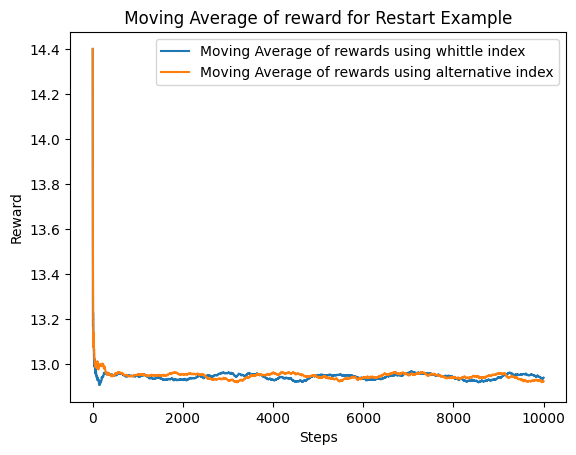
\includegraphics[scale=0.5]{comparison_A_homo_restart.png}
% \caption{Approach A: N=100,M=20}
\begin{center}
\begin{tabular}{cc}
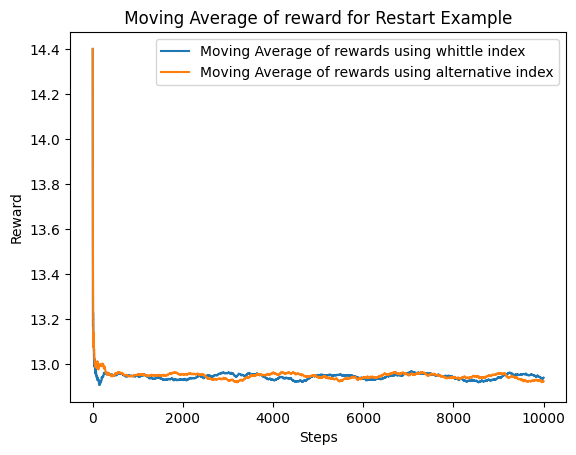
\includegraphics[scale=0.6]{comparison_A_homo_restart.png} &
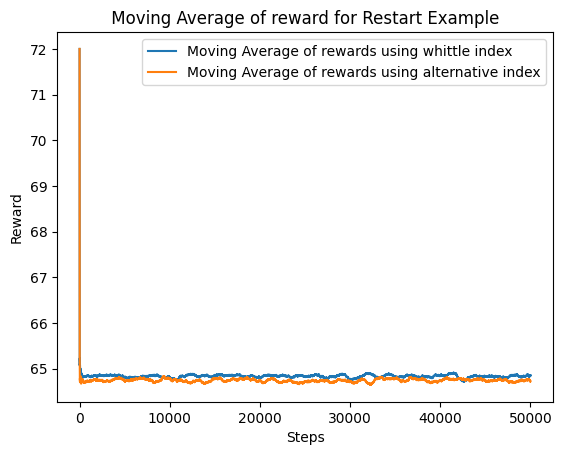
\includegraphics[scale=0.6]{Moving Average of reward for Restart Example_final.png} \\
\begin{small}
 Approach A: N=20, M=4\end{small} & \begin{small}Approach B, N=100, M=20\end{small}\\
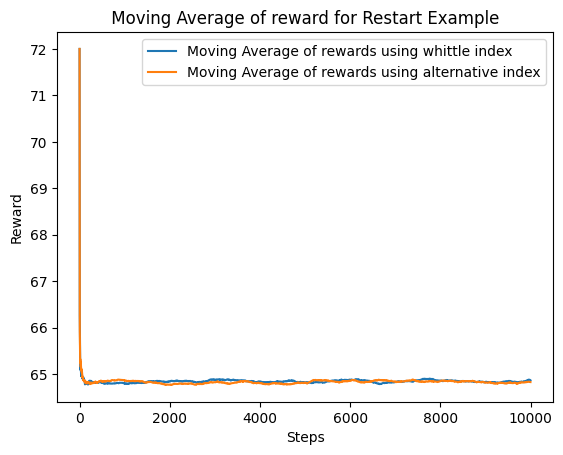
\includegraphics[scale=0.6]{homo_restart_compariosn_C.png} &
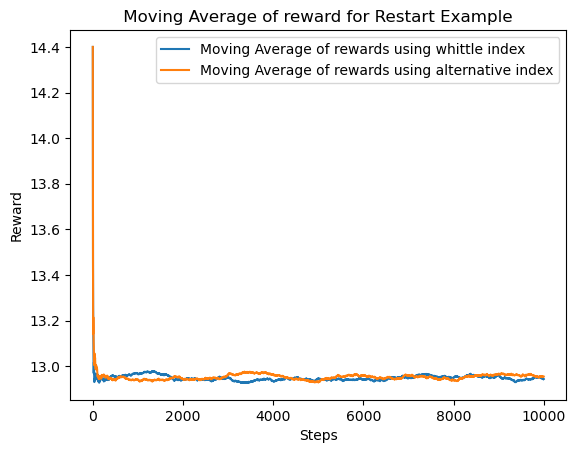
\includegraphics[scale=0.6]{comparison_homo_restart_D.png} \\
\begin{small}
 Approach C: N=20, M=4\end{small} & \begin{small}Approach D, N=100, M=20\end{small}\\
 \end{tabular}

\end{center}
    
\newpage
\textbf{Calculating Lagrange indices using DDQN}
\begin{algorithm}[H]
\begin{small}
\begin{algorithmic}[1]
    \State Initialize $\lambda^*$, primary Q network $Q_\theta$, Target Q network $Q_{\theta'}$, Batch Size,$\epsilon$=1.

    % \Function{VisualizationRecommendation}{$B$, $D$, $M$}:
    % \State $\epsilon \gets \text{initialize an error value for terminate condition}$
    % \State $S \gets [S_1, S_2, S_3, ...., S_{
    % |S|}]$  $\text{($|S_{k+1}| > |S_{k}|$ $\forall k \in [1, |S| - 1]$)}$
    % \State $m$ $\gets$ $\text{number of columns of $S_k$}$
    % \State $n$ $\gets$ $\text{number of features per column}$
    \For {n\;=\;1:\;$n_{end}$}
        
        \State Update $\beta(n)$ as:
        $\beta(n)=\frac{1}{\lceil{nlog(n)\backslash5000}\rceil+1}$
        \For{arm $i\in N$}
            \State Choose action $a_{n}^i$ for  arm i in an $\epsilon$-greedy fashion
            \State Update $s_{n+1}^i$ and reward $r_n^i$ from $s_{n}^i$ and $a_{n}^i$ for  arm i
            \State Store $(s_{n}^i,a_{n}^i,r_{n}^i,s_{n+1}^i,\lambda_n^*)$ in experience replay buffer
            \State Train DQN policy model on one batch of $(s_{n},a_{n},r_{n},s_{n+1},\lambda_n^*)$ tuples from experience replay buffer using:
            \Statex\begin{small}
            $Q_{target}(s_n,a_n)\gets(1-a_n)(r_o(s_n)+\lambda_n^*)+a_nr_1(s_n)+\underset{v\epsilon\{0,1\}}{max}Q_{\theta'}(s_{n+1},v)-\frac{1}{2d}\sum\limits_{k\in S}Q_{\theta}(k,0)+Q_{\theta}(k,1)$\end{small}
            % \State Update ($s_n^i$,$a_n^i$) Q-values for each arm i as:
            % \Statex\begin{small}$Q_{n+1}(s_n,a_n)\gets(1-\alpha(n))Q_n(s_n,a_n)+\alpha(n)((1-a_n)(r_o(s_n)+\lambda_n^*)+a_nr_1(s_n)+\underset{v\epsilon\{0,1\}}{max}Q_n(s_{n+1},v)-\frac{1}{2d}\sum\limits_{k\in S}Q_n(k,0)+Q_n(k,1))$\end{small}
        \EndFor
        \State Update the Target Q network 
        \State Update common subsidy for passivity for all arms $\lambda^*$ as: $\lambda_{n+1}^*=\lambda_n^*+\beta(n)(\sum\limits_{i=1}^{i=N}a_n^i-M)$
        
        \State Decrement $\epsilon$ as $\epsilon_{n+1}=max(0.01,\epsilon_{n}*0.99)$
        % \State $total \textunderscore cost \gets 0$
        % \State $\Tilde{y_{k}} \gets$ \text{ranking score of the viz produced using all the features predicted by P}
        % \State $terminate \textunderscore flag \gets False$
        % \While{not $terminate \textunderscore flag$}
        %     \If{$random$ in $[0,1) \leq Pr_{\text {rand}}$} 
        %         \State $ij \gets$ \text{index of a randomly selected unknown feature}
        %     \Else
        %         \State $ij$ $\gets$ $Q(x^{k, t})$ $\text{(index of the feature with the maximum Q value)}$
        %     \EndIf
        %     \State $x^{k, t+1} \gets \text{acquire $f_{ij}$ and unmask it}$
        %     \State $P(x^{k, t}) \gets \text{ranking score predicted using the feature set $x^{k, t}$}$
        %     \State $total \textunderscore cost \gets total \textunderscore cost +\boldsymbol{c}_{\boldsymbol{ij}}$ 
        %     \State $r_{ij}^{k, t} \leftarrow \frac{\left\|\operatorname{P}\left(\boldsymbol{x}^{k,t}\right)-\operatorname{P}\left(\boldsymbol{x}^{k, t+1}\right)\right\|}{\boldsymbol{c}_{ij}} $
        %     \State \text{push} $\left(\boldsymbol{x^{k, t}}, \boldsymbol{x^{k, t+1}}, ij, r_{ij}^{k, t}, \tilde{y_k}\right)$ \text{into the replay memory}
        %     \State $t \leftarrow t+1$
        %     \If{$total \textunderscore cost \geq B$}
        %         \State $terminate \textunderscore flag \gets True$
        %         \State $\hat{y_k} \gets P(x^{k, t})   \text{predicted viz ranking  score on subset of features $x^{k, t}$}$
        %     \EndIf
        %     \State \text{loss} $\gets$ $L(\Tilde{y_k}$,$\hat{y_k})$
        %     \If{$update \textunderscore condition$}
        %         \State \text{train \textunderscore batch} $\gets$ \text{random mini-batch from the replay memory}
        %         \State \text{update Q and target Q networks using train batch }
        %     \EndIf
                
        % \EndWhile
        % \If{$\epsilon > loss$}
        %     terminate loop
        % \EndIf
        
    \EndFor
    \State Calculate the new index for every state s of each arm i by:
        \Statex\hspace*{5mm} $\delta(s)=Q_{\theta}(s,1)-Q_{\theta}(s,0)$
\end{algorithmic}
\end{small}
\end{algorithm}
\newpage
\begin{center}
    
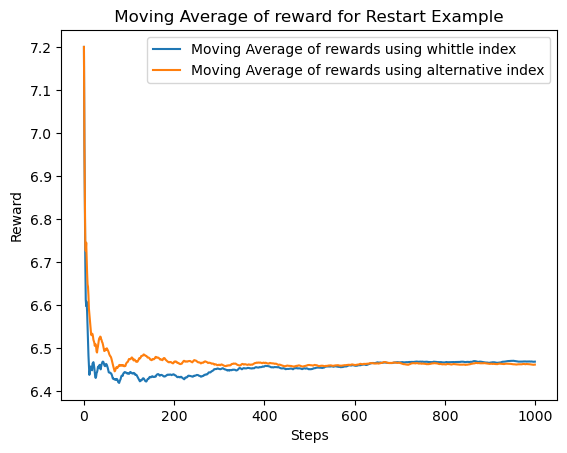
\includegraphics[scale=0.75]{restart_dqn.png}
\end{center}

\begin{center}
    
\begin{small}
\vspace{-10mm}
\hspace{5mm}DDQN: N=10, M=2\end{small}

 \end{center}
\newpage
\textbf{Non Whittle Indexable Example}\\
The following problem  is a Non-Whittle Indexable problem. The transition probability matrices are: 
 \begin{align*}
P_0=
\begin{bmatrix}
0.005 & 0.793 & 0.202\\
0.027 & 558 & 0.415 \\
0.736&0.249&0.015
\end{bmatrix}
\hspace{1mm} \text{and} \hspace{1mm}
P_1=
\begin{bmatrix}
0.718 & 0.254 & 0.028\\
0.347 & 0.097 & 0.556 \\
0.015&0.956&0.029
\end{bmatrix}
\end{align*}
With the Reward Matrix: $[0,0.699],[0,0.362],[0,0.715]$\\
In many Non-Whittle Indexable problems, Whittle Indices are used empirically. Hence
even we calculate the Whittle Indices for this problem and compare the performance of our indices against
them.

\newpage
\begin{center}
\begin{tabular}{cc}
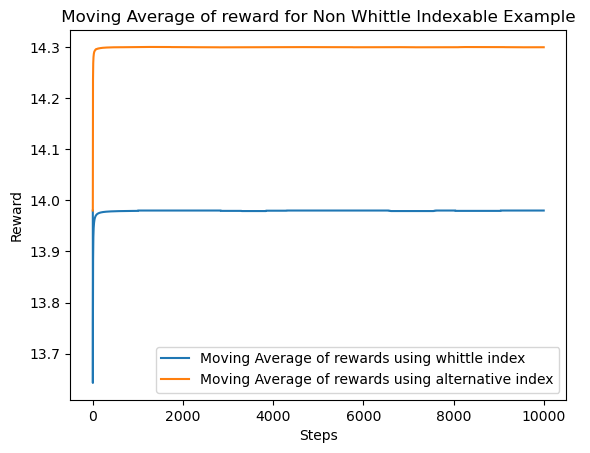
\includegraphics[scale=0.6]{non_whittle_comparison_A.png} &
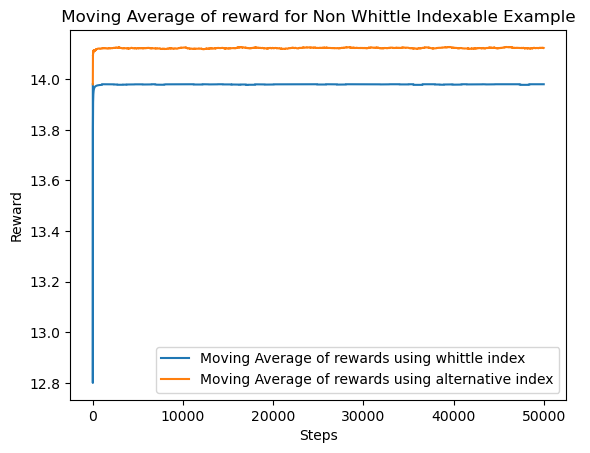
\includegraphics[scale=0.6]{reward_non_whittle.png} \\
\begin{small}
 Approach A: N=100, M=20\end{small} & \begin{small}Approach B, N=100, M=20\end{small}\\
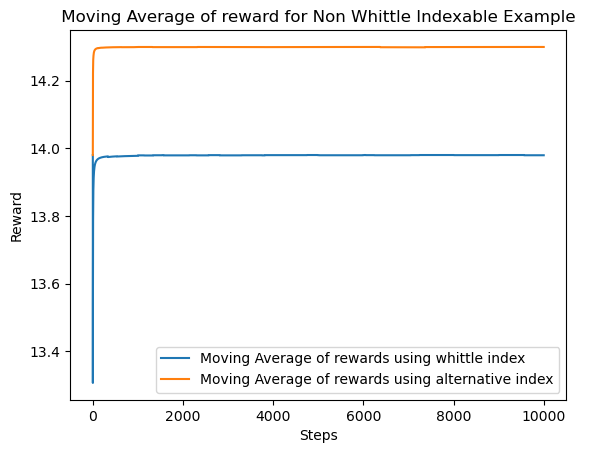
\includegraphics[scale=0.6]{non_whittle_comparison_C.png} &
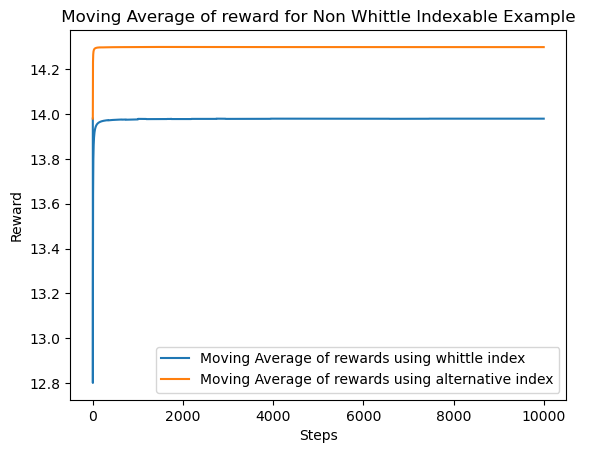
\includegraphics[scale=0.6]{non_whittle_comparison_D.png} \\
\begin{small}
 Approach C: N=100, M=20\end{small} & \begin{small}Approach D, N=100, M=20\end{small}\\
 \end{tabular}

\end{center}
\newpage
\vspace{.75in}
\begin{center}
\textit{\textbf{\LARGE \color{red} THANK YOU! }}
\end{center}
}

\end{document}

